\documentclass[9pt]{beamer}

\usepackage{booktabs}
\usepackage{multirow}
\usepackage{array}
\usepackage{makecell}
\usepackage{graphicx}
\usepackage{fancyhdr}
\usepackage{svg}
\usepackage{amsmath}
\usepackage{hyperref}
\usepackage{url}
\usepackage{physics}
\usepackage{amssymb}
\usepackage{float}
\usepackage{subcaption} % loads the caption package

\usepackage{pgfplots}
\pgfplotsset{compat=1.18}
\usetikzlibrary{positioning,arrows.meta}

\usepackage{algorithm}
\usepackage{algpseudocode}

\usepackage{wrapfig}
\usepackage{minted}
\usepackage{xcolor}
\usepackage{media9}
\usepackage{multimedia}  % For embedding videos
% \usepackage[backend=biber,style=numeric]{biblatex} % Adjust style as needed
\hypersetup{
    colorlinks=true,
    linkcolor=blue,
    filecolor=magenta,      
    urlcolor=blue,
}
% Theme and customization
\usetheme{default} % Change this to try different themes
\usecolortheme{beaver} % Change color scheme as needed
\setbeamertemplate{navigation symbols}{} % Remove navigation symbols

% Title and author information
\title{Integer Factorization as an Ising problem}
% \subtitle{Optional Subtitle}
\author{Anil Prabhakar, Advith Desu, Aryan Namboodri}
\institute{Indian Institute of Technology Madras}
\date{\today}

\begin{document}

% Title slide
\begin{frame}
    \begin{tikzpicture}[remember picture, overlay]
        \node[anchor=north west, xshift=0.6cm, yshift=-0.4cm]
            at (current page.north west)
            {
\includegraphics[height=1.3cm]{iitm_logo.png}};
        \node[anchor=north east, xshift=-0.6cm, yshift=-0.4cm]
            at (current page.north east)
            {
\includegraphics[height=1.6cm]{cquicc_logo.png}};
    \end{tikzpicture}
    \titlepage
\end{frame}


%====================================================
\section{Introduction}
%====================================================

\begin{frame}{Factorization Problem}
\begin{itemize}
\item Given a natural number $N$, find $P,Q$ such that
\[
N = P Q
\]
\item Hard inverse problem underlying RSA security.
\item Map factorization $\rightarrow$ QUBO (or Ising) problem.
\item Solve using annealing-based algorithms.
\end{itemize}
\end{frame}

%====================================================
\section{Formulation}
%====================================================

\begin{frame}{Binary Representation and Assumptions}
Assumptions:
\begin{itemize}
\item $N$ is odd.
\item Factors have equal bit-length
\[
n=\left\lceil \tfrac12 \log_2 N \right\rceil.
\]
\end{itemize}

Binary form:
\[
P=\sum_{k=0}^{n-1}2^k p_k,\quad
Q=\sum_{k=0}^{n-1}2^k q_k,\quad p_k,q_k\in\{0,1\}.
\]

Fixed bits:
\[
p_0=q_0=1,\qquad p_{n-1}=q_{n-1}=1.
\]
\end{frame}

\begin{frame}{Column-wise Multiplication}
\begin{itemize}
\item Construct binary long multiplication table.
\item Introduce carry variables $s_{i,j}$.
\item Each column gives a constraint:
\[
C_i = N_i - \sum_{j} q_j p_{i-j}
      - \sum s_{j,i}
      + \sum 2^j s_{i,i+j}.
\]
\item Correct factors satisfy $C_i = 0$.
\end{itemize}
\end{frame}

\begin{frame}{Energy Function}
Optimization objective:
\[
\min_{\{p_i,q_i,s_{ij}\}} \sum_i (C_i)^2.
\]

\begin{itemize}
\item Binary variables: factor bits + carry bits.
\item Ground state corresponds to valid factorization.
\item Alternative direct method:
\[
\left(N-\sum p_i2^i \sum q_j2^j\right)^2
\]
but gives fewer preprocessing opportunities.
\end{itemize}
\end{frame}

%====================================================
\section{Classical Pre-processing}
%====================================================

\begin{frame}{Rule 1: Saturated Sum}
For binary $x_i \in \{0,1\}$:
\[
\sum_{i=1}^{n} x_i = n \quad\Longrightarrow\quad x_i = 1 \ \forall i.
\]

\textbf{Why:} the only way $n$ binary variables sum to $n$ is for every one of them to be $1$.

\medskip
A symmetric form with negative coefficients:
\[
\sum_{i=1}^{n} -x_i = -n \quad\Longrightarrow\quad x_i = 1 \ \forall i.
\]
\end{frame}

\begin{frame}{Rule 2: Zero Sum}
For binary $x_i \in \{0,1\}$:
\[
\sum_{i=1}^{n} x_i = 0 \quad\Longrightarrow\quad x_i = 0 \ \forall i.
\]

\textbf{Why:} a sum of non-negative binaries equals $0$ only when every term is $0$.

\medskip
The same conclusion holds with negative coefficients:
\[
\sum_{i=1}^{n} -x_i = 0 \quad\Longrightarrow\quad x_i = 0 \ \forall i.
\]
\end{frame}

\begin{frame}{Rule 3: Doubling Rule}
For binary variables $x_1, x_2, x_3 \in \{0,1\}$:
\[
x_1 + x_2 = 2 x_3 \quad\Longrightarrow\quad x_1 = x_2 = x_3.
\]

\textbf{Why:} LHS $\in \{0,1,2\}$ and RHS $\in \{0,2\}$. Equality forces LHS even, so $x_1+x_2 \in \{0,2\}$ — both equal, and equal to $x_3$.

\medskip
\textbf{Use in factorization:} appears whenever a column clause has only two factor-bit terms balanced against a single carry, e.g.
\[
p_k + q_k = 2 s \;\Rightarrow\; p_k = q_k = s.
\]
\end{frame}

\begin{frame}{Rule 4: Coefficient Bound Rule}
General linear constraint on $x_i \in \{0,1\}$:
\[
\sum_i c_i x_i + C = 0,\qquad
S_+ \!=\! \sum_{c_i>0} c_i,\quad S_- \!=\! \sum_{c_j<0} |c_j|.
\]

If a single coefficient is larger than the max possible opposing sum, the variable is \emph{forced}:

\smallskip
\textbf{Positive coefficients} ($c_i > 0$):
\[
c_i > S_- - C \;\Rightarrow\; x_i = 0,\qquad
c_i > S_+ + C \;\Rightarrow\; x_i = 1.
\]

\textbf{Negative coefficients} ($c_j < 0$, $|c_j|$ magnitude):
\[
|c_j| > S_+ + C \;\Rightarrow\; x_j = 0,\qquad
|c_j| > S_- - C \;\Rightarrow\; x_j = 1.
\]

\textbf{Example:} $x_1 + x_2 = 2x_3 + 1$. Coefficient of $x_3$ is $2$, max LHS is $2$, so $x_3$ cannot be $1$ $\Rightarrow x_3 = 0$.
\end{frame}

\begin{frame}{Rule 5: Complement Rule}
For binary $x_1, x_2 \in \{0,1\}$:
\[
x_1 + x_2 = 1 \quad\Longrightarrow\quad x_2 = 1 - x_1, \quad x_1 x_2 = 0.
\]

\textbf{Why:} the only solutions are $(0,1)$ and $(1,0)$ — exactly one variable is $1$, so their product is always $0$.

\medskip
\textbf{Use in factorization:} eliminates one variable outright (substitute $x_2 \to 1-x_1$) and kills any quadratic term $x_1 x_2$ that appears in a column clause.
\end{frame}

\begin{frame}{Parity Rule}
Both sides of a clause must have the same parity:
\begin{align*}
x_1 + x_2 + \text{even} &= \text{even} \;\Rightarrow\; x_1 = x_2, \\[3pt]
x_1 + x_2 + \text{even} &= \text{odd}  \;\Rightarrow\; x_1 + x_2 = 1.
\end{align*}

\textbf{Example:}
\[
x_1 + x_2 + 2x_3 = 2y_1 + 4y_2 \;\Rightarrow\; x_1 = x_2,
\]
\[
x_1 + x_2 + 2x_3 = 2y_1 + 4y_2 + 1 \;\Rightarrow\; x_1 + x_2 = 1.
\]

\medskip
\textbf{Why it matters:} column clauses balance a small sum of factor bits against carries with even coefficients ($2 s_{i,i+1},\ 4 s_{i,i+2},\dots$). The parity of the factor-bit sum is therefore locked by $N_i$.
\end{frame}

\begin{frame}{Power Rule}
For any binary variable $x \in \{0,1\}$:
\[
x^m = x, \quad m = 2, 3, \dots
\]

\textbf{Why:} $0^m = 0$ and $1^m = 1$ for all positive integers $m$.

\medskip
\textbf{Use in factorization:} after squaring the energy function $E = \sum_i C_i^2$, every $p_k^2,\ q_k^2,\ s^2$ collapses back to its linear form $p_k,\ q_k,\ s$. This is what makes the squared objective expressible as a (degree-2) QUBO once cubics/quartics are quadrized.
\end{frame}


%=================================================

\begin{frame}{Worked Example: $N = 391 = 17 \times 23$}

\textbf{Setup:}
\begin{itemize}
  \item $391 = 110000111_2$
  \item \textbf{Fixed bits:} $p_0 = q_0 = 1$ (odd), $p_4 = q_4 = 1$ (MSB)
  \item \textbf{Free bits:} $p_1, p_2, p_3$ and $q_1, q_2, q_3$ — 6 unknowns
\end{itemize}

\medskip
\textbf{Long multiplication table} (cross-product $p_a q_b$ sits in column $a+b$):

\begin{center}
\scriptsize
\setlength{\tabcolsep}{4pt}
\renewcommand{\arraystretch}{1.4}
\begin{tabular}{|c|c|c|c|c|c|c|c|c|c|}
\hline
 & $2^8$ & $2^7$ & $2^6$ & $2^5$ & $2^4$ & $2^3$ & $2^2$ & $2^1$ & $2^0$ \\
\hline
$P$ &     &     &     &     & 1     & $p_3$ & $p_2$ & $p_1$ & 1     \\
$Q$ &     &     &     &     & 1     & $q_3$ & $q_2$ & $q_1$ & 1     \\
\hline
        &     &     &     &     & 1     & $p_3$ & $p_2$ & $p_1$ & 1 \\
        &     &     &     & $q_1$ & $p_3 q_1$ & $p_2 q_1$ & $p_1 q_1$ & $q_1$ &  \\
        &     &     & $q_2$ & $p_3 q_2$ & $p_2 q_2$ & $p_1 q_2$ & $q_2$ &     &     \\
        &     & $q_3$ & $p_3 q_3$ & $p_2 q_3$ & $p_1 q_3$ & $q_3$ &     &     &     \\
        & 1   & $p_3$ & $p_2$ & $p_1$ & 1     &     &     &     &     \\
\hline
Carry-ins  & $s_{6,8},s_{7,8}$ & $s_{5,7},s_{6,7}$ & $s_{4,6},s_{5,6}$ & $s_{3,5},s_{4,5}$ & $s_{2,4},s_{3,4}$ & $s_{2,3}$ & $s_{1,2}$ & & \\
\hline
Carry-outs & & $s_{7,8}$ & $s_{6,7},s_{6,8}$ & $s_{5,6},s_{5,7}$ & $s_{4,5},s_{4,6}$ & $s_{3,4},s_{3,5}$ & $s_{2,3},s_{2,4}$ & $s_{1,2}$ & \\
\hline
$N=391$ & \textbf{1} & \textbf{1} & \textbf{0} & \textbf{0} & \textbf{0} & \textbf{0} & \textbf{1} & \textbf{1} & \textbf{1} \\
\hline
\end{tabular}
\end{center}

Carry $s_{i,j}$ = bit of column $i$'s carry destined for column $j$ (coefficient $2^{j-i}$). In each $C_k$, positive-sign carries enter column $k$ (\textbf{carry-ins}); negative-sign carries with weights $2,4,\dots$ leave column $k$ (\textbf{carry-outs}).
\end{frame}

\begin{frame}{Column Clauses: $C_i = 0$}

\small
Each column $i$: $(\text{column sum}) + (\text{carries in}) = N_i + 2 s_{i,i+1} + 4 s_{i,i+2}$.

\medskip
\begin{align*}
C_0 &:\ 1 - 1 = 0 \quad \checkmark\\
C_1 &:\ p_1 + q_1 - 1 - 2 s_{1,2} = 0 \\
C_2 &:\ p_2 + q_2 + p_1 q_1 + s_{1,2} - 1 - 2 s_{2,3} - 4 s_{2,4} = 0 \\
C_3 &:\ p_3 + q_3 + p_1 q_2 + p_2 q_1 + s_{2,3} - 2 s_{3,4} - 4 s_{3,5} = 0 \\
C_4 &:\ 2 + p_1 q_3 + p_3 q_1 + p_2 q_2 + s_{2,4} + s_{3,4} - 2 s_{4,5} - 4 s_{4,6} = 0 \\
C_5 &:\ p_1 + q_1 + p_2 q_3 + p_3 q_2 + s_{3,5} + s_{4,5} - 2 s_{5,6} - 4 s_{5,7} = 0 \\
C_6 &:\ p_2 + q_2 + p_3 q_3 + s_{4,6} + s_{5,6} - 2 s_{6,7} - 4 s_{6,8} = 0 \\
C_7 &:\ p_3 + q_3 + s_{5,7} + s_{6,7} - 1 - 2 s_{7,8} = 0 \\
C_8 &:\ 1 + s_{6,8} + s_{7,8} - 1 = 0
\end{align*}
\end{frame}

\begin{frame}{Applying Reduction Rules}
\small

\textbf{$C_8$ (Rule 2, sum $= 0$):} $s_{6,8} + s_{7,8} = 0 \Rightarrow \boxed{s_{6,8} = s_{7,8} = 0}$.

\medskip
\textbf{$C_2$ (Rule 4, large coefficient):} LHS terms $p_2{+}q_2{+}p_1q_1{+}s_{1,2} \le 4$, but coefficient of $s_{2,4}$ is $4$. If $s_{2,4}{=}1$, need LHS $\ge 5$. \quad $\boxed{s_{2,4} = 0}$.

\medskip
\textbf{$C_1$ (Rule 5):} $p_1 + q_1 = 1 + 2 s_{1,2}$. Max sum $= 2 < 3$, so $s_{1,2} = 0$:
\[
\boxed{s_{1,2} = 0,\quad q_1 = 1 - p_1} \quad\Rightarrow\quad p_1 q_1 = p_1(1-p_1) = 0
\]

\medskip
\textbf{$C_2$ (after substitutions):} $p_2 + q_2 = 1 + 2 s_{2,3}$.\ Same logic as $C_1$:
\[
\boxed{s_{2,3} = 0,\quad q_2 = 1 - p_2}
\]

\medskip
\textbf{$C_7$ (Rule 2, sum $= 1$ exactly-one):}
\[
p_3 + q_3 + s_{5,7} + s_{6,7} = 1 \quad (s_{7,8}=0 \text{ already})
\]
Exactly one of these four binaries equals 1.
\end{frame}

\begin{frame}{Remaining Structure After Pre-processing}
\small

After the rules above, we have eliminated $5$ variables ($s_{1,2}, s_{2,3}, s_{2,4}, s_{6,8}, s_{7,8}$) and reduced $q_1, q_2$ to functions of $p_1, p_2$.

\medskip
\textbf{Free QUBO variables (13):}
\[
\{p_1, p_2, p_3, q_3\} \cup \{s_{3,4}, s_{3,5}, s_{4,5}, s_{4,6}, s_{5,6}, s_{5,7}, s_{6,7}\}
\quad (\text{plus } 2 \text{ auxiliaries from quadrization})
\]

\textbf{Remaining clauses} (after substituting $q_1{=}1{-}p_1,\ q_2{=}1{-}p_2$):
\begin{align*}
C_3 &:\ p_3 + q_3 + p_1(1{-}p_2) + p_2(1{-}p_1) - 2 s_{3,4} - 4 s_{3,5} = 0 \\
    &\ \ = p_3 + q_3 + p_1 + p_2 - 2 p_1 p_2 - 2 s_{3,4} - 4 s_{3,5} = 0 \\
C_4 &:\ 2 + p_1 q_3 + p_3(1{-}p_1) + p_2(1{-}p_2) + s_{3,4} - 2 s_{4,5} - 4 s_{4,6} = 0 \\
    &\ \ = 2 + p_1 q_3 + p_3 - p_1 p_3 + s_{3,4} - 2 s_{4,5} - 4 s_{4,6} = 0 \\
C_5 &:\ 1 + p_2 q_3 + p_3(1{-}p_2) + s_{3,5} + s_{4,5} - 2 s_{5,6} - 4 s_{5,7} = 0 \\
C_6 &:\ 1 + p_3 q_3 + s_{4,6} + s_{5,6} - 2 s_{6,7} = 0 \\
C_7 &:\ p_3 + q_3 + s_{5,7} + s_{6,7} = 1
\end{align*}

\textbf{Cubic terms appear} after squaring (e.g.\ $p_1 p_2 \cdot s_{3,4}$ in $C_3^2$, $p_1 p_3 \cdot s_{4,5}$ in $C_4^2$) $\Rightarrow$ \textbf{quadrization required}.
\end{frame}

\begin{frame}{Quadrization and QUBO Construction}
\small

\textbf{Energy function:} $E = \sum_{i=3}^{7} C_i^2$. Squaring introduces cubics like $a\cdot p_i p_j s_{k,\ell}$.

\medskip
\textbf{Rosenberg substitution:} replace each $AB$ pair appearing in a cubic by an auxiliary $w$, with penalty
\[
P(A,B,w) = M\bigl(AB - 2Aw - 2Bw + 3w\bigr),\qquad M \gg \max\,|\text{coeff}|.
\]
$P=0$ iff $w = AB$. After substitution every cubic $A B \cdot s$ becomes $w \cdot s$ (quadratic).

\medskip
\textbf{Auxiliaries needed:} $w_1 = p_1 p_2,\ w_2 = p_1 p_3$.

\medskip
\textbf{Full QUBO:}
\[
H = \sum_{i=3}^{7} C_i^2 \Big|_{w_1 \to p_1 p_2,\, w_2 \to p_1 p_3}
\;+\; M\bigl[P(p_1,p_2,w_1) + P(p_1,p_3,w_2)\bigr]
\]

\textbf{Active QUBO variables (13 total):}
\begin{center}
\begin{tabular}{ll}
\toprule
Original (4) & $p_1,\ p_2,\ p_3,\ q_3$ \\
Carry (7)    & $s_{3,4},\ s_{3,5},\ s_{4,5},\ s_{4,6},\ s_{5,6},\ s_{5,7},\ s_{6,7}$ \\
Auxiliary (2) & $w_1 = p_1 p_2,\ w_2 = p_1 p_3$ \\
\bottomrule
\end{tabular}
\end{center}
\end{frame}

\begin{frame}{QUBO Matrix Structure}
\small

\textbf{Sketch of nonzero entries} of $Q$ for $N=391$ (after pre-processing and quadrization):

\begin{center}
\scriptsize
\begin{tabular}{l|cccc|ccccccc|cc}
\toprule
        & $p_1$ & $p_2$ & $p_3$ & $q_3$ & $s_{3,4}$ & $s_{3,5}$ & $s_{4,5}$ & $s_{4,6}$ & $s_{5,6}$ & $s_{5,7}$ & $s_{6,7}$ & $w_1$ & $w_2$ \\
\midrule
$p_1$    & $\bullet$ & $\bullet$ & $\bullet$ & $\bullet$ & & & & & & & & $\bullet$ & $\bullet$ \\
$p_2$    &   & $\bullet$ & $\bullet$ & $\bullet$ & $\bullet$ & $\bullet$ & & & & & & $\bullet$ &   \\
$p_3$    &   &   & $\bullet$ & $\bullet$ & $\bullet$ & & $\bullet$ & $\bullet$ & & & $\bullet$ &   & $\bullet$ \\
$q_3$    &   &   &   & $\bullet$ & & & $\bullet$ & $\bullet$ & $\bullet$ & $\bullet$ & $\bullet$ & & \\
\midrule
$s_{3,4}$ & & & & & $\bullet$ & $\bullet$ & $\bullet$ & $\bullet$ & & & & & \\
$s_{3,5}$ & & & & & & $\bullet$ & $\bullet$ & & $\bullet$ & $\bullet$ & & & \\
$s_{4,5}$ & & & & & & & $\bullet$ & $\bullet$ & $\bullet$ & $\bullet$ & & & \\
$s_{4,6}$ & & & & & & & & $\bullet$ & $\bullet$ & & $\bullet$ & & \\
$s_{5,6}$ & & & & & & & & & $\bullet$ & $\bullet$ & $\bullet$ & & \\
$s_{5,7}$ & & & & & & & & & & $\bullet$ & $\bullet$ & & \\
$s_{6,7}$ & & & & & & & & & & & $\bullet$ & & \\
\midrule
$w_1$    & & & & & & & & & & & & $\bullet$ & \\
$w_2$    & & & & & & & & & & & & & $\bullet$ \\
\bottomrule
\end{tabular}
\end{center}

The ground state of this QUBO recovers $P{=}17,\,Q{=}23$ with $E{=}0$.

\end{frame}

%====================================================
\section{From QUBO to Ising}
%====================================================

\begin{frame}{QUBO $\rightarrow$ Ising Conversion}

QUBO uses $x_i \in \{0,1\}$; Ising-form annealers (D-Wave, our GPU SA) use spins $\sigma_i \in \{-1,+1\}$.

\medskip
\textbf{Linear change of variables:}
\[
\sigma_i = 1 - 2 x_i \qquad\Longleftrightarrow\qquad x_i = \tfrac{1 - \sigma_i}{2}.
\]

\medskip
Substitute into the QUBO $H = \sum_i Q_{ii}\,x_i + \sum_{i<j} Q_{ij}\,x_i x_j$ and collect terms:
\[
H(\boldsymbol\sigma) = \underbrace{\sum_i h_i \sigma_i}_{\text{linear field}} \;+\; \underbrace{\sum_{i<j} J_{ij}\,\sigma_i \sigma_j}_{\text{couplings}} \;+\; \text{const}.
\]

\textbf{Coefficients} (treating $Q$ symmetrically so $Q_{ij}=Q_{ji}$ for $i\neq j$):
\[
\boxed{\,J_{ij} = \tfrac{1}{4} Q_{ij}\,},\qquad
\boxed{\,h_i = -\tfrac{1}{2} Q_{ii} \;-\; \tfrac{1}{4}\sum_{j\neq i} Q_{ij}\,}.
\]

\end{frame}


\begin{frame}[allowframebreaks]{J matrix Visualization}

    \begin{figure}[htp]
        \centering
        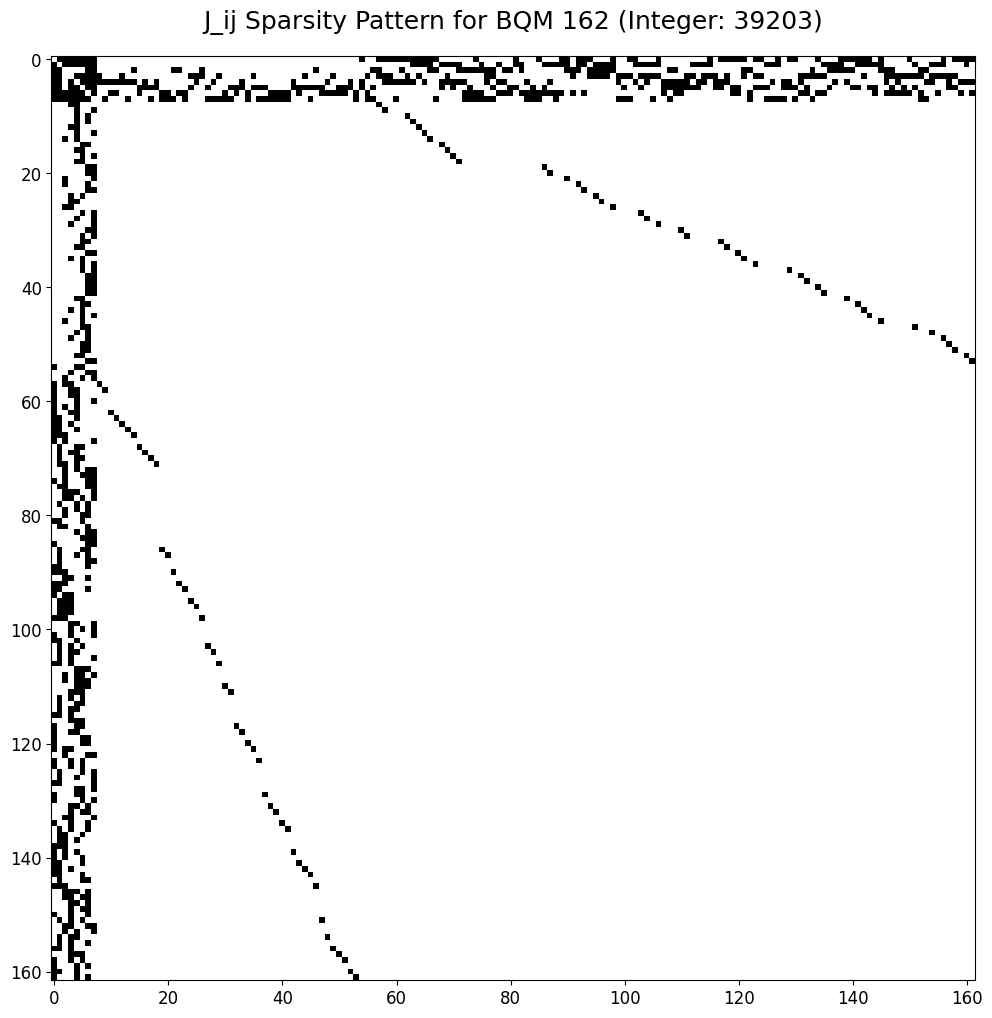
\includegraphics[width=0.62\textwidth]{Sparsity of J matrix for 162 BQM.png}
        \caption{Sparsity of $J$ matrix for 162 spins (Integer 39203).}
        \label{fig: Sparsity of J matrix for 162 spins (Integer 39203).}
    \end{figure}

    \begin{figure}[htp]
        \centering
        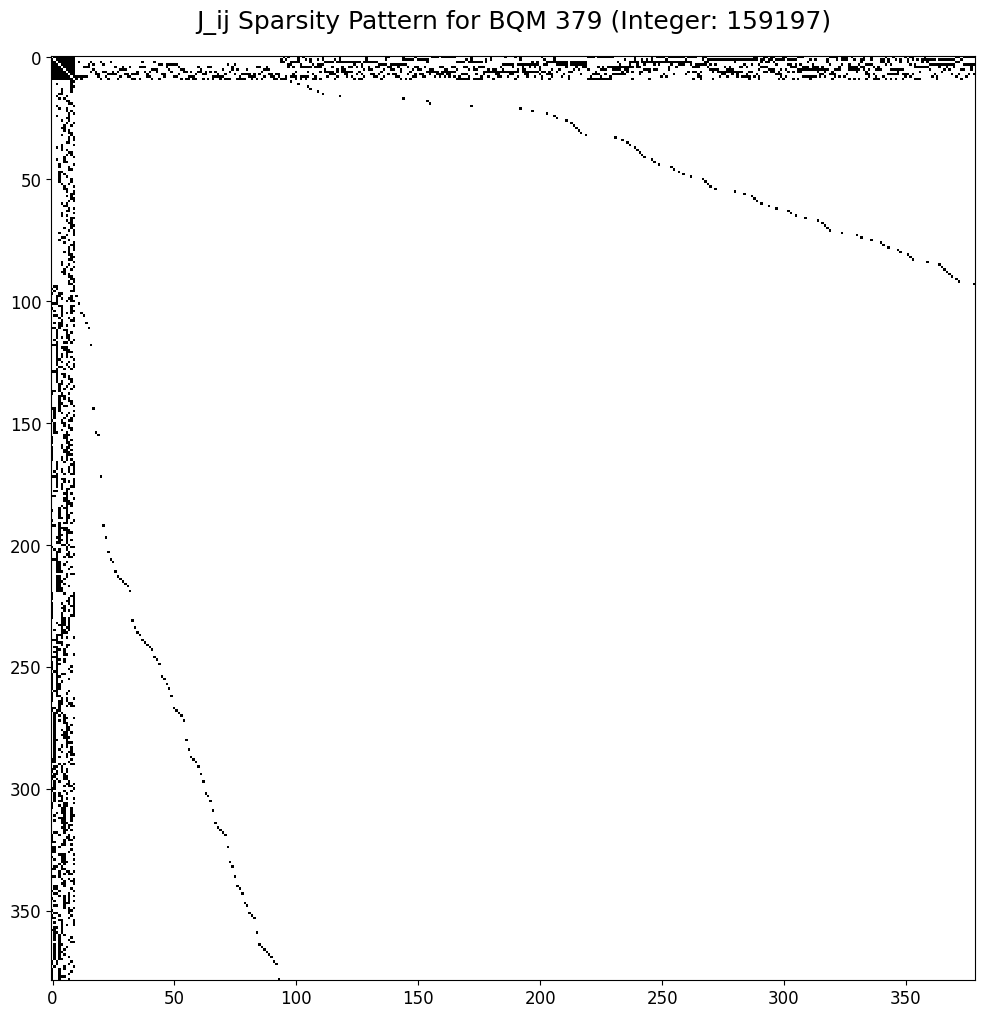
\includegraphics[width=0.62\textwidth]{Sparsity of J matrix for 379 BQM.png}
        \caption{Sparsity of $J$ matrix for 379 spins (Integer 159197).}
        \label{fig: Sparsity of J matrix for 379 spins (Integer 159197).}
    \end{figure}

    \begin{figure}[htp]
        \centering
        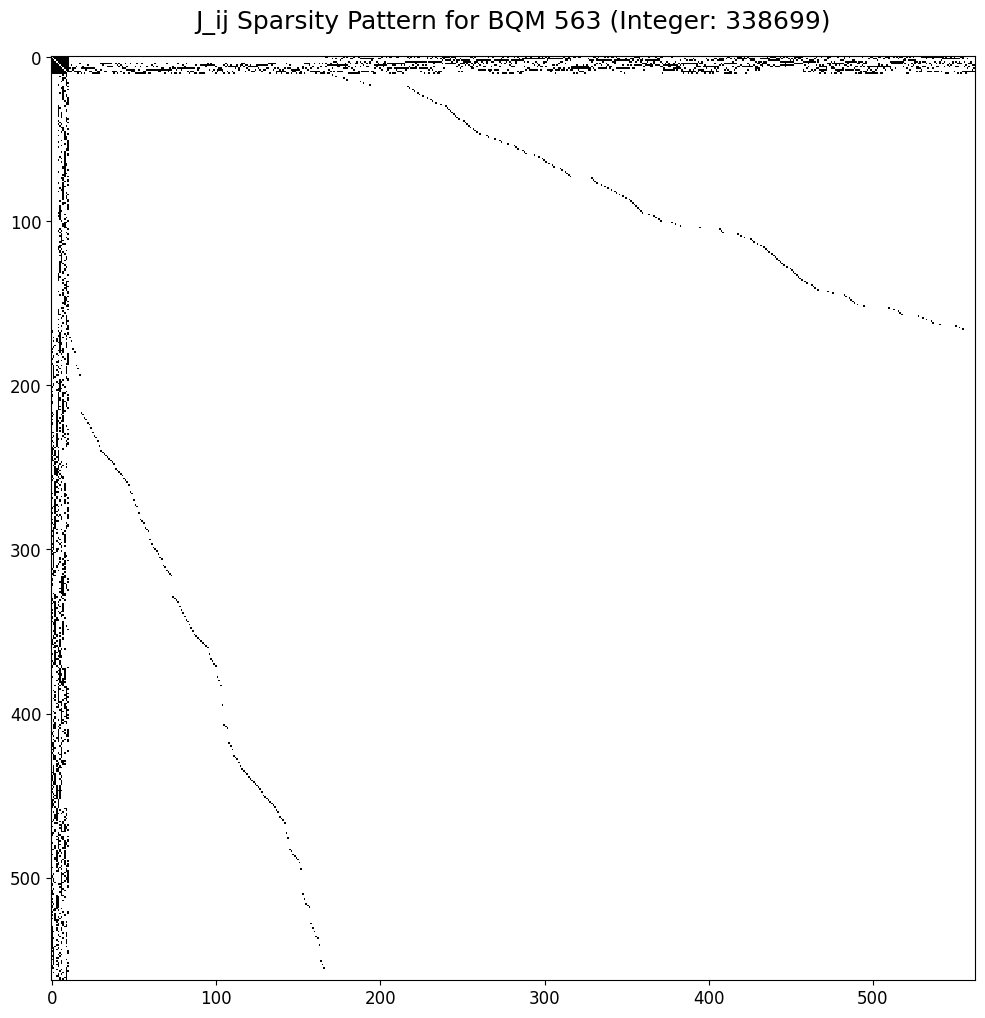
\includegraphics[width=0.62\textwidth]{Sparsity of J matrix for 563 BQM.png}
        \caption{Sparsity of $J$ matrix for 563 spins (Integer 338699).}
        \label{fig: Sparsity of J matrix for 563 spins (Integer 338699).}
    \end{figure}

\end{frame}

\begin{frame}{Sparse Coupling Matrix Representation (CSR)}

\textbf{Problem:}
The Ising coupling matrix $J_{ij}$ is very large but mostly zero.
Storing it as a dense $N \times N$ matrix wastes memory and bandwidth.

\vspace{0.3cm}
\textbf{Key idea:}
Store \emph{only the nonzero couplings} using
\alert{Compressed Sparse Row (CSR)} format. CSR represents a sparse matrix using three arrays:

\[
\texttt{row\_ptr}[i] \quad \text{start index of row } i
\]
\[
\texttt{col\_idx}[k] \quad \text{column index of nonzero entry}
\]
\[
\texttt{values}[k] \quad \text{value of } J_{ij}
\]

Only nonzero entries are stored.

\vspace{0.2cm}
\textbf{Memory cost:} $\mathcal{O}(N + \text{nnz})$ instead of $\mathcal{O}(N^2)$ (nnz = number of nonzeros).

\end{frame}

\begin{frame}{CSR Example}

Consider a symmetric $5 \times 5$ coupling matrix with $8$ non-zero entries (out of $25$):

\medskip
\begin{minipage}{0.42\textwidth}
\centering
\[
J =
\begin{pmatrix}
\cdot &  2  & \cdot & \cdot & -1 \\
 2  & \cdot & \cdot &  3  & \cdot \\
\cdot & \cdot & \cdot & \cdot &  4  \\
\cdot &  3  & \cdot & \cdot & \cdot \\
-1  & \cdot &  4  & \cdot & \cdot
\end{pmatrix}
\]
{\scriptsize ($\cdot$ denotes a stored zero — not represented in CSR)}
\end{minipage}%
\hfill
\begin{minipage}{0.55\textwidth}
\textbf{CSR representation:}

\smallskip
\scriptsize
\setlength{\tabcolsep}{4pt}
\renewcommand{\arraystretch}{1.3}
\begin{tabular}{l|*{9}{c}}
index               & 0 & 1 & 2 & 3 & 4 & 5 & 6 & 7 & \\
\hline
\texttt{col\_idx} & 1 & 4 & 0 & 3 & 4 & 1 & 0 & 2 & \\
\texttt{values}   & 2 & -1 & 2 & 3 & 4 & 3 & -1 & 4 & \\
\end{tabular}

\medskip
\begin{tabular}{l|*{6}{c}}
index              & 0 & 1 & 2 & 3 & 4 & 5 \\
\hline
\texttt{row\_ptr}[i] & 0 & 2 & 4 & 5 & 6 & 8 \\
\end{tabular}
\end{minipage}

\medskip
\textbf{Reading row $i$:} entries in row\_ptr[i] represent the start of the $i^{\text{th}}$ row in the J values array. Entries are stored at indices $\texttt{row\_ptr}[i] \dots \texttt{row\_ptr}[i{+}1]{-}1$ of the column index.

\vspace{0.2cm}
\textbf{Memory cost:} $\mathcal{O}(N + \text{nnz})$ instead of $\mathcal{O}(N^2)$ (nnz = number of nonzeros).

\end{frame}

\begin{frame}{GPU Kernel}

    \bigskip

    \begin{figure}[htp]
        \centering
        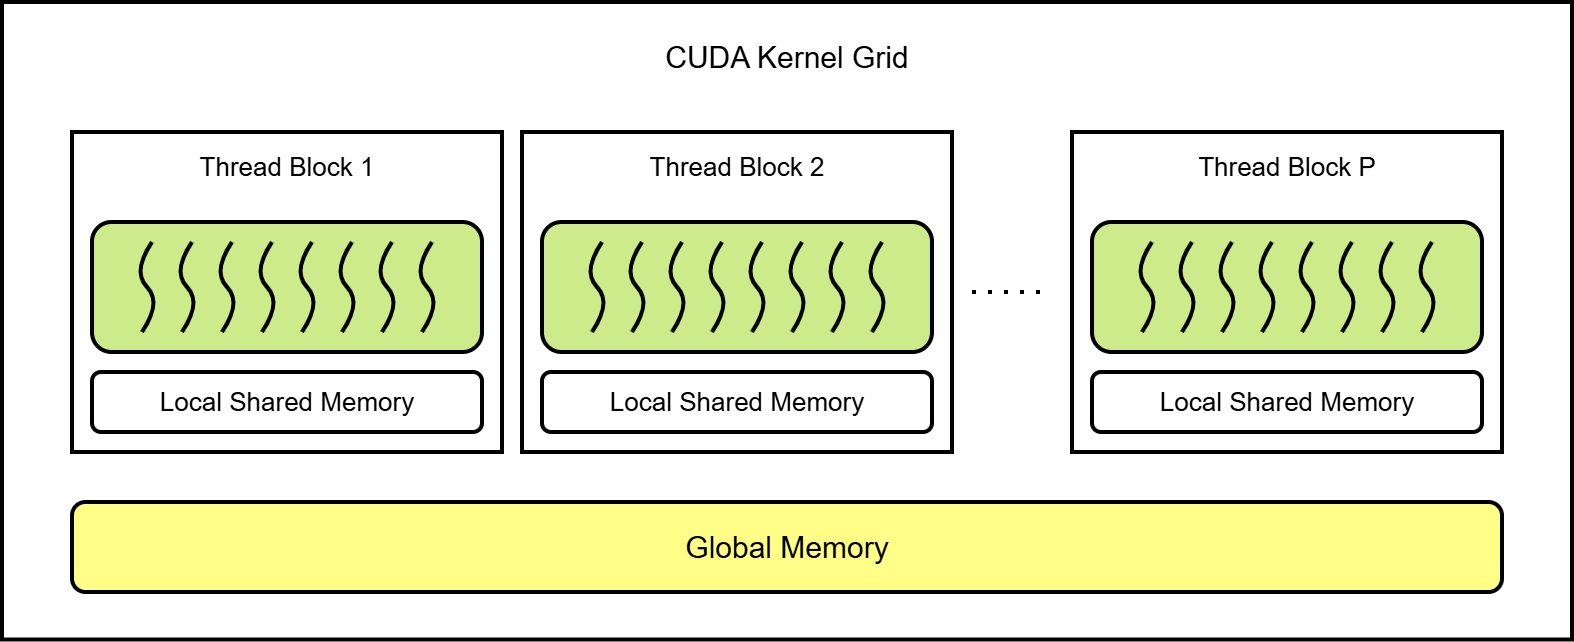
\includegraphics[width=0.85\textwidth]{GPU Threads.png}
        \caption{GPU Threads and Thread blocks.}
        \label{fig: GPU Threads and Thread blocks.}
    \end{figure}
    
\end{frame}

\begin{frame}{GPU Thread Calculation in DA1}

    Each thread $i$ calculates the local field $L_i = \sum_j J_{ij}s_j + h_i$ and the energy difference is then calculated as $-2 \times s_i \times L_i$ depending on which $i^{\text{th}}$ spin flipped.

    \begin{figure}[htp]
        \centering
        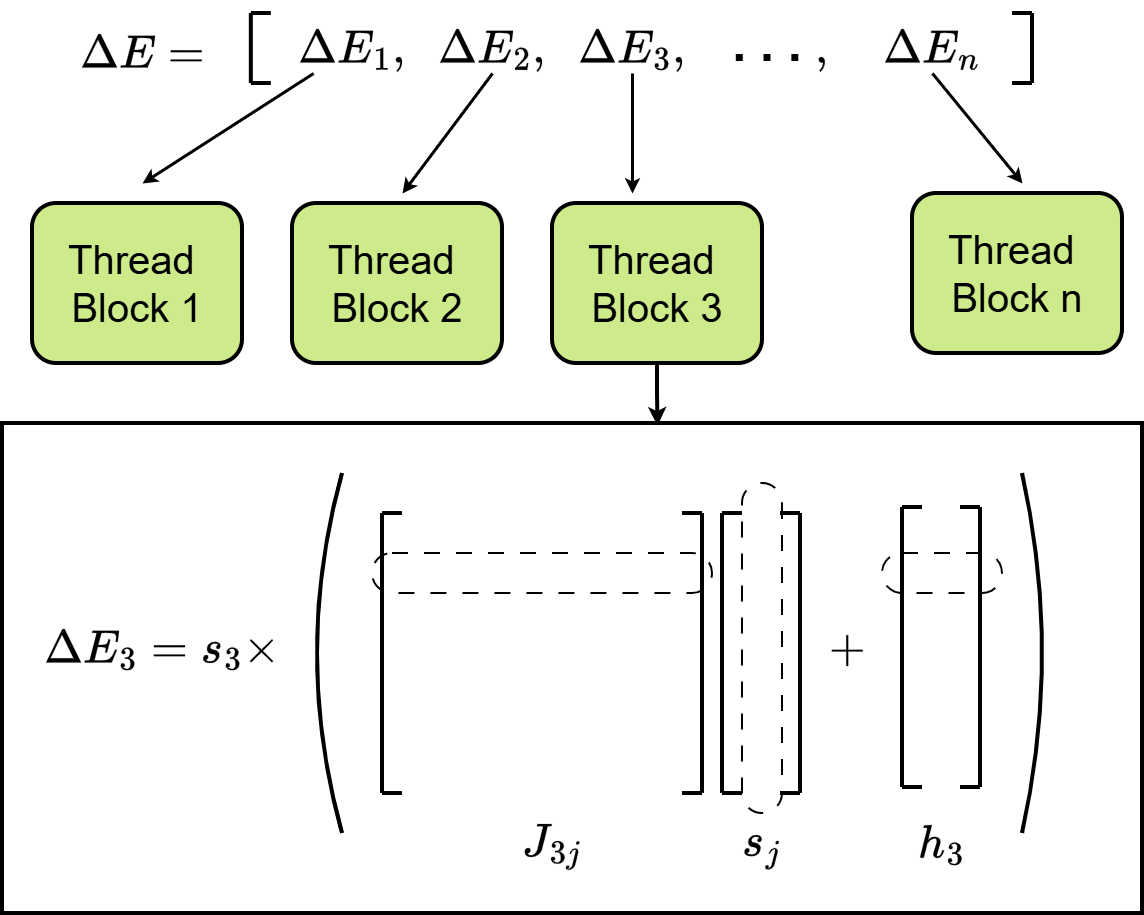
\includegraphics[width=0.65\textwidth]{Energy calculation in DA1.png}
        \caption{Energy calculation in DA1.}
        \label{fig: Energy calculation in DA1.}
    \end{figure}
    
\end{frame}

\begin{frame}{Graph-Coloring Simulated Annealing}

In one Metropolis sweep we want to flip many spins in parallel, but two spins coupled by a non-zero $J_{ij}$ share an edge and cannot be flipped simultaneously without invalidating each other's $\Delta E$.

\medskip
We use graph coloring on the interaction graph (nodes = spins, edges = nonzero $J_{ij}$) partitions spins into colors such that \emph{no two same-color spins are coupled}. All spins in one color can then be flipped in parallel without affecting each other's energy calculations.

\medskip
\textbf{Two performance bins} based on row degree $d_i = |\{j : J_{ij} \neq 0\}|$:
\begin{itemize}
  \item \textbf{Dense} ($d_i \ge 128$): full block of $1024$ threads, shared-memory reduction.
  \item \textbf{Sparse} ($d_i < 128$): one warp (32 threads) per spin, $32$ spins packed per block, warp-shuffle reduction.
\end{itemize}
\end{frame}

\begin{frame}{Number of Total and Densely Connected Spins with Scale}

    \begin{figure}[htp]
        \centering
        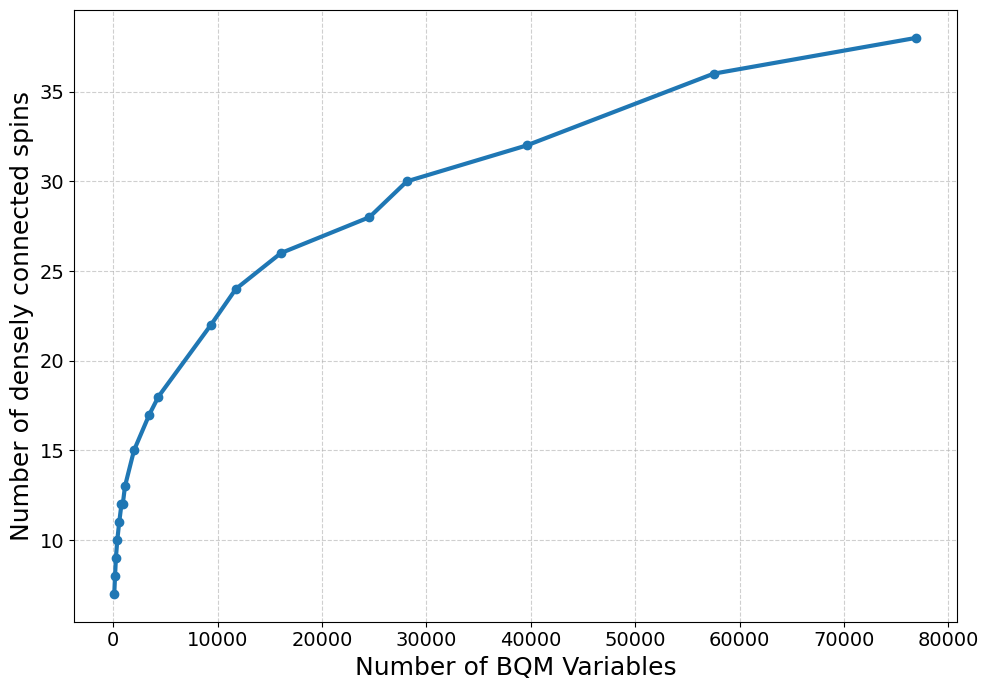
\includegraphics[width=0.9\textwidth]{bqm variables vs number of densely connected spins.png}
        \caption{Number of bits in N vs number of densely connected spins.}
        \label{fig: bqm variables vs number of densely connected spins.}
    \end{figure}
    
\end{frame}

\begin{frame}{One-time Setup}

\begin{algorithm}[H]
\caption{Pre-processing steps before annealing}
\begin{algorithmic}[1]
\Require CSR of symmetric $J$, linear field $h$, num\_spins $N$
\State Verify $J$ symmetry and a zero diagonal
\State Bin each spin: \textbf{dense} if $d_i \ge 128$, else \textbf{sparse}
\State $\text{color}[\,] \gets$ Welsh--Powell greedy coloring (largest-degree-first, first-fit)
\State Bucket spins by color: \texttt{color\_dense\_offsets}, \texttt{color\_sparse\_offsets}
\State Upload all CSR + color tables + hub arrays to GPU
\State Initialize a random spin configuration and compute initial energy
\State Calculate the start-temperature: $T_0 = \langle \Delta E^+ \rangle / \ln(1/\chi)$ \newline ($\chi$ = target acceptance rate)
\end{algorithmic}
\end{algorithm}

\end{frame}

\begin{frame}{Annealing Loop (GPU)}

\begin{algorithm}[H]
\caption{Color-parallel simulated annealing}
\begin{algorithmic}[1]
\Require $\beta$-schedule $\{\beta_t\}$ (geometric), sweeps per $\beta$, $N_{\text{colors}}$
\For{$\beta$ in $\beta$-schedule}
  \For{sweep $= 1 \ldots m$}
    \State Generate fresh uniform randoms for all $N$ spins
    \For{$c = 0 \ldots N_{\text{colors}} - 1$} \Comment{colors run sequentially}
      \State \textbf{collectFlipCandidates}$\langle$dense$\rangle$ on color $c$ 
      \State \textbf{collectFlipCandidates}$\langle$sparse$\rangle$ on color $c$
      \State \quad each spin $i$ in color $c$ \textbf{in parallel}:
      \State \quad\quad $L_i \gets \sum_j J_{ij}s_j + h_i$, $\Delta E_i \gets -2 s_i L_i$
      \State \quad\quad if $\text{rand}_i < \min(1, e^{-\beta\Delta E_i})$: append $(i, \Delta E_i)$ to candidates
      \State \textbf{applyAllFlipsInColor}: flip every accepted spin, atomicAdd $\Delta E_i$ to total energy
      \State if any hub spin in color $c$: refresh hub-values cache
    \EndFor
  \EndFor
  \If{total energy $<$ best energy} snapshot best spins \EndIf
\EndFor
\State \Return best-energy spin configuration
\end{algorithmic}
\end{algorithm}

\end{frame}


%========================================

\begin{frame}{Annealing Time per Iteration vs Number of Spins}

    \begin{figure}
        \centering
        \includegraphics[width=0.9\linewidth]{spins_vs_time_per_iteration_for_mac_gh200.png}
    \end{figure}

\end{frame}

\begin{frame}{Time Taken for Construction and Annealing}

    \begin{figure}
        \centering
        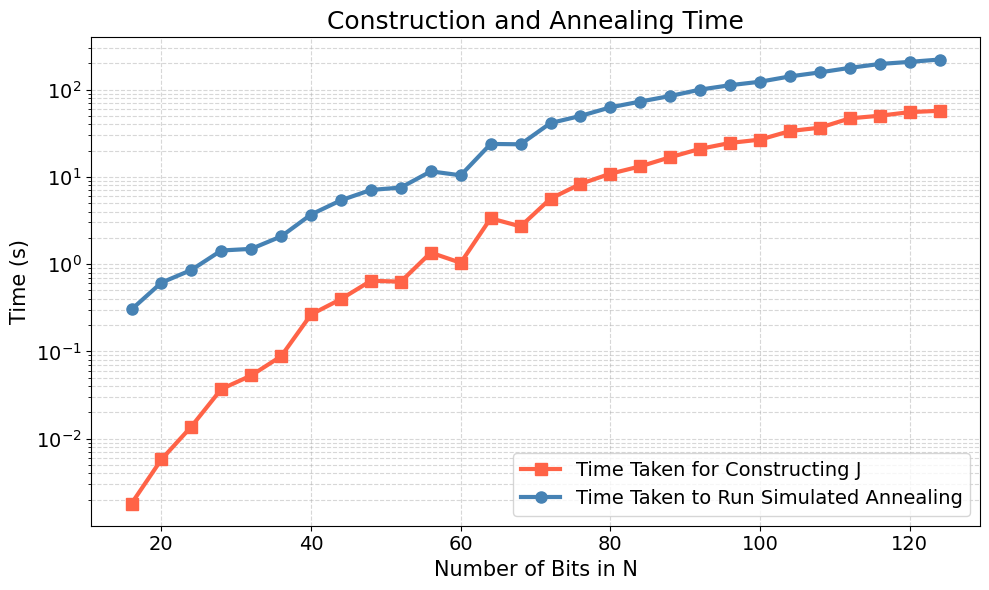
\includegraphics[width=\linewidth]{Construction and Annealing Time.png}
    \end{figure}

    Each Annealing run consists of 10 sweeps at each temperature step, with the starting temperature $T_0$ calculated to give an initial acceptance rate of 0.5, and a geometric cooling schedule with factor 0.95 until $T < 10^{-3}$.

\end{frame}

\begin{frame}{Solution Quality Measured by Gap between Real and Estimated P}

    \begin{figure}
        \centering
        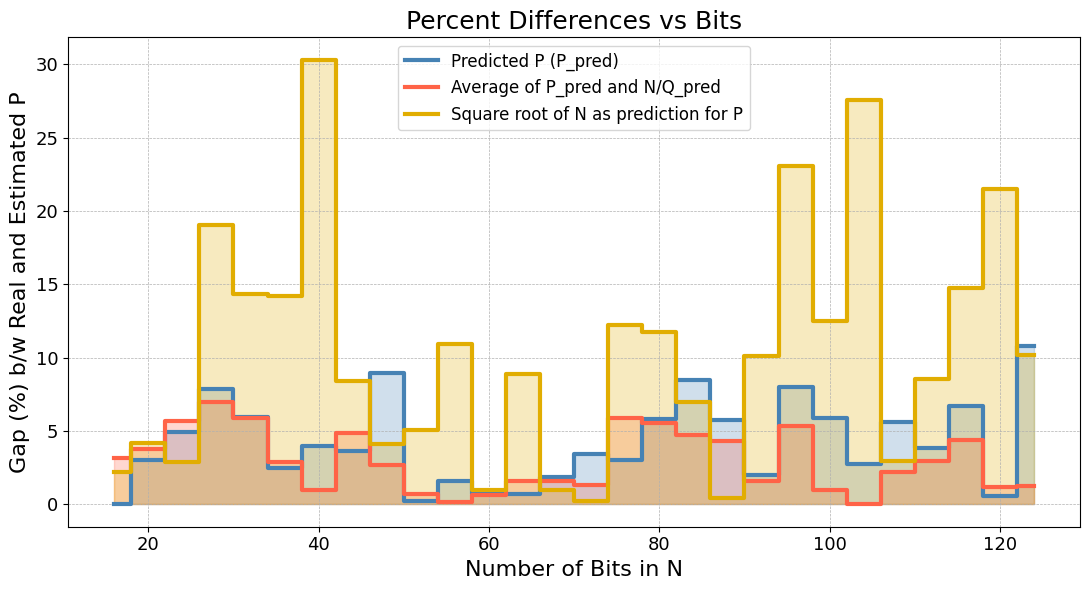
\includegraphics[width=1\linewidth]{Percentage Gap between real and estimated P.png}
    \end{figure}

    \begin{enumerate}
        \item Average (\%) difference with square root N as the estimate = \textbf{10.33\%}
        \item Average (\%) difference with $P_{\text{pred}}$ from Simulated Annealing = \textbf{4.23\%}
        \item Average (\%) difference with mean of $P_{\text{pred}}$ and $N / Q_{\text{pred}}$ = \textbf{2.98\%}
    \end{enumerate}

\end{frame}

%====================================================
\section{Brute-force Search}
%====================================================

\begin{frame}{Brute-force Search}

The annealer returns approximate factors $P_{\text{pred}}, Q_{\text{pred}}$ — usually off by a few percent. A brute-force search around this prediction finds the exact factor.

\medskip
\textbf{Best starting estimate} — average of two independent guesses for $P$:
\[
P_{\text{centre}} \;=\; \tfrac{1}{2}\bigl(P_{\text{pred}} + \lfloor N / Q_{\text{pred}} \rfloor\bigr).
\]

\medskip
\textbf{Outward spiral:} test candidates closest to $P_{\text{centre}}$ first, alternating above and below until the exact factor is found.

\medskip
Candidates are grouped into chunks of $C$. Even chunks spiral upward (steps up), odd chunks spiral downward (steps down). Threads claim the next chunk via an atomic counter, so the search is partially parallel.

\medskip
\textbf{Stop condition:} the first thread to find $p \mid N$ sets a shared flag; the rest exit at the next iteration.

\end{frame}

\begin{frame}{Brute-force Optimizations}

Testing all numbers in a chunk is ineffecient as we can filter out many candidates without a divisibility test using a wheel sieve cheaply. The wheel sieve eliminates candidates that are divisible by small primes.

\medskip
\textbf{Wheel Sieve:}
\begin{itemize}
  \item Any $p$ divisible by $2, 3, 5, 7,$ or $11$ cannot be the (odd, $\ge 13$) prime factor.
  \item Using a Wheel sieve skips approximately 79\% of candidates without a divisibility test.
\end{itemize}

\medskip
\textbf{Early termination:} atomic \texttt{stop} flag checked at each chunk boundary; all $T$ threads exit within one chunk of the discovery.

\end{frame}

\begin{frame}{Brute-force Algorithm}

\begin{algorithm}[H]
\caption{Parallel spiral divisor search}
\begin{algorithmic}[1]
\Require $N,\ P_{\text{pred}},\ Q_{\text{pred}},\ T$ threads
\State $P_{\text{centre}} \gets \tfrac{1}{2}(P_{\text{pred}} + \lfloor N/Q_{\text{pred}} \rfloor)$
\State \textbf{shared:} atomic \texttt{chunk\_idx} $\gets 0$, atomic \texttt{stop} $\gets$ false, atomic \texttt{found} $\gets 0$
\medskip
\For{each thread \textbf{in parallel}}
  \While{\textbf{not} \texttt{stop}}
    \State $k \gets$ \texttt{chunk\_idx.fetchAdd(1)} \Comment{claim next chunk}
    \If{$k$ even} \Comment{step up}
      \State $[\text{lo},\text{hi}] \gets [P_{\text{centre}} + \tfrac{k}{2}C,\ P_{\text{centre}} + (\tfrac{k}{2}{+}1)C - 1]$
    \Else \Comment{step down}
      \State $[\text{lo},\text{hi}] \gets [P_{\text{centre}} - \tfrac{k{+}1}{2}C,\ P_{\text{centre}} - \tfrac{k{-}1}{2}C - 1]$
    \EndIf
    \For{each $p \in [\text{lo}, \text{hi}]$ passing the wheel sieve}
      \If{$N \bmod p = 0$}
        \State \texttt{found} $\gets p$;\ \texttt{stop} $\gets$ true;\ \textbf{return}
      \EndIf
    \EndFor
  \EndWhile
\EndFor
\State \Return $P \gets$ \texttt{found},\ \ $Q \gets N / P$
\end{algorithmic}
\end{algorithm}
\end{frame}

\begin{frame}{Time Taken to Find Exact primes by Brute Force}

    \begin{figure}
        \centering
        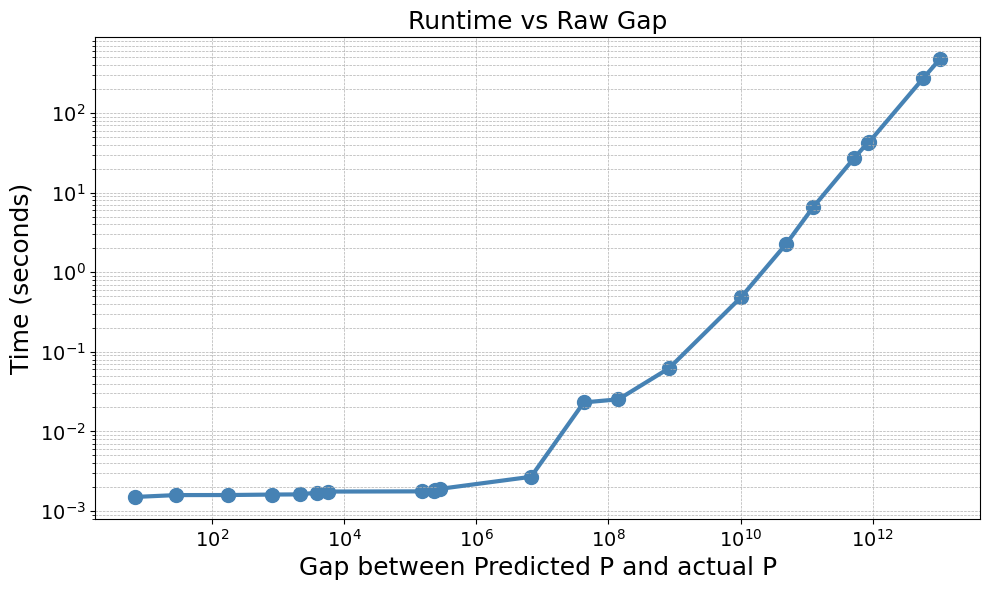
\includegraphics[width=1\linewidth]{Raw gap vs Time taken to find solution.png}
    \end{figure}

    $$\text{Time Taken (s)} = \frac{3.32 \times 10^{-9}}{\text{Threads}} \times \text{Gap (\%)} \times 2^n$$

\end{frame}

\begin{frame}{End-to-End Run: $\sim$100-bit Semiprime}

\[
N \;=\; 416\,749\,328\,744\,899\,275\,664\,046\,210\,629
\]

\bigskip
\begin{center}
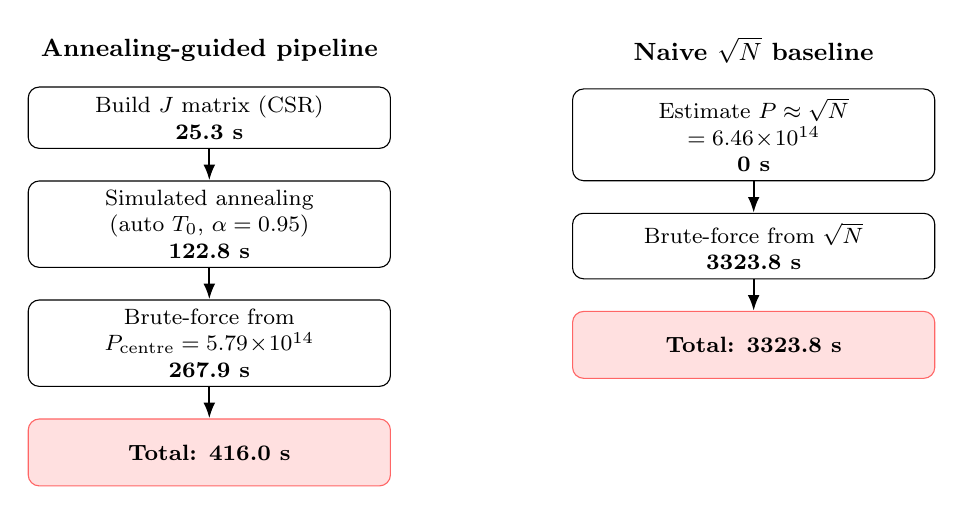
\begin{tikzpicture}[
  node distance=4mm,
  box/.style={draw, rounded corners, minimum width=4.6cm, minimum height=0.7cm,
              align=center, font=\footnotesize},
  total/.style={draw, rounded corners, minimum width=4.6cm, minimum height=0.85cm,
                align=center, font=\footnotesize\bfseries, fill=red!12, draw=red!60},
  hdr/.style={font=\small\bfseries},
  arr/.style={-{Latex[length=2mm]}, thick}
]
% ===== Left column: annealing pipeline =====
\node[hdr] (lh) {Annealing-guided pipeline};
\node[box, below=2mm of lh]   (l1) {Build $J$ matrix (CSR) \\ \textbf{25.3 s}};
\node[box, below=of l1]       (l2) {Simulated annealing \\ (auto $T_0$, $\alpha = 0.95$) \\ \textbf{122.8 s}};
\node[box, below=of l2]       (l3) {Brute-force from \\ $P_{\text{centre}} = 5.79\!\times\!10^{14}$ \\ \textbf{267.9 s}};
\node[total, below=of l3]     (l4) {Total: \textbf{416.0 s}};
\draw[arr] (l1) -- (l2);
\draw[arr] (l2) -- (l3);
\draw[arr] (l3) -- (l4);

% ===== Right column: sqrt(N) baseline =====
\node[hdr, right=3.0cm of lh] (rh) {Naive $\sqrt{N}$ baseline};
\node[box, below=2mm of rh]   (r1) {Estimate $P \approx \sqrt{N}$ \\ $= 6.46\!\times\!10^{14}$ \\ \textbf{0 s}};
\node[box, below=of r1]       (r2) {Brute-force from $\sqrt{N}$ \\ \textbf{3323.8 s}};
\node[total, below=of r2]     (r3) {Total: \textbf{3323.8 s}};
\draw[arr] (r1) -- (r2);
\draw[arr] (r2) -- (r3);

\end{tikzpicture}
\end{center}

\medskip
\centerline{\small Factors found: $P = 573\,858\,364\,692\,161,\ \ Q = 726\,223\,323\,360\,389$ \quad (72 threads)}
\centerline{The annealer's prediction places the brute-force search much closer to the true factor.}

\end{frame}

%====================================================
\section{Future Work}
%====================================================

\begin{frame}{Future Work}

\textbf{Better classical post-processing.} Brute-force trial division is the simplest way to consume the annealer's guess $(P_{\text{pred}}, Q_{\text{pred}})$, but it makes almost no use of the prediction beyond using it as a starting point. Other Existing classical factorization methods may be able to exploit this kind of information far more effectively than a linear scan. Exploring such methods would be a natural next step.

\medskip
\textbf{The Bottleneck}, from the brute-force timing model
\[
\text{Time}(\text{s}) \;=\; \frac{3.32 \times 10^{-9}}{\text{threads}} \,\times\, \text{Gap}(\%) \,\times\, 2^n,
\]

\begin{itemize}
  \item \textbf{Threads:} This is the amount of 'compute' we can throw at the problem. Would be helpful, but its bounded by hardware.
  \item \textbf{Gap (\%):} a multiplicative factor in front of $2^n$. Since $2^n$ grows exponentially with bit-length, \emph{shrinking the gap helps us keep up} with larger $N$.
\end{itemize}

\medskip
\textbf The next step would be to improve the solution quality from the annealer by exploring better QUBO encodings, and any other optimizations that drives $P_{\text{pred}}$ closer to $P$ and chips away at the $\text{Gap}(\%)$.

\end{frame}

%====================================================
\section{References}
%====================================================

\begin{frame}{References}
\small
\begin{thebibliography}{9}

\bibitem{wang2020}
B.~Wang, F.~Hu, H.~Yao, and C.~Wang,
``Prime factorization algorithm based on parameter optimization of Ising model,''
\emph{Scientific Reports}, vol.~10, no.~1, 2020.
DOI: \href{https://doi.org/10.1038/s41598-020-62802-5}{10.1038/s41598-020-62802-5}.

\bibitem{jiang2018}
S.~Jiang, K.~A. Britt, A.~J. McCaskey, T.~S. Humble, and S.~Kais,
``Quantum Annealing for Prime Factorization,''
\emph{Scientific Reports}, vol.~8, no.~1, 2018.
DOI: \href{https://doi.org/10.1038/s41598-018-36058-z}{10.1038/s41598-018-36058-z}.

\bibitem{preis2009}
T.~Preis, P.~Virnau, W.~Paul, and J.~J. Schneider,
``GPU accelerated Monte Carlo simulation of the 2D and 3D Ising model,''
\emph{Journal of Computational Physics}, vol.~228, no.~12, pp.~4468--4477, 2009.
DOI: \href{https://doi.org/10.1016/j.jcp.2009.03.018}{10.1016/j.jcp.2009.03.018}.

\end{thebibliography}

\end{frame}


\end{document}
